% FitDash — agent / MCP-server radial architecture (standalone, crops to figure).
% Orchestrator at the centre, 5 specialist agents around it, each wired out to the
% MCP server(s) it uses (server name big, its tools small). Fitness uses a RAG
% store rather than an MCP server. Inner ring = Agent Layer, outer ring = Tool Layer.
% Build:  latexmk -pdf fitdash-agents-radial.tex
\documentclass[border=12pt]{standalone}
\usepackage[T1]{fontenc}
\usepackage[sfdefault]{FiraSans}
\usepackage{xcolor}
\usepackage{tikz}
\usetikzlibrary{backgrounds,arrows.meta}

\definecolor{fdNavy}{HTML}{0B1219}
\definecolor{fdSlate}{HTML}{16212B}
\definecolor{fdBorder}{HTML}{1E293B}
\definecolor{fdTeal}{HTML}{2DD4BF}
\definecolor{fdTealDark}{HTML}{14B8A6}
\definecolor{fdMuted}{HTML}{64748B}

% Never hyphenate tool names mid-word (e.g. "cre-ate_event"); wrap only at commas.
\hyphenpenalty=10000
\exhyphenpenalty=10000
\tolerance=9999
\emergencystretch=3em

% Server box: big bold name on top, small muted tool list below.
\newcommand{\srv}[2]{{\large\bfseries #1}\\[2pt]{\scriptsize\textcolor{fdMuted}{#2}}}

\begin{document}
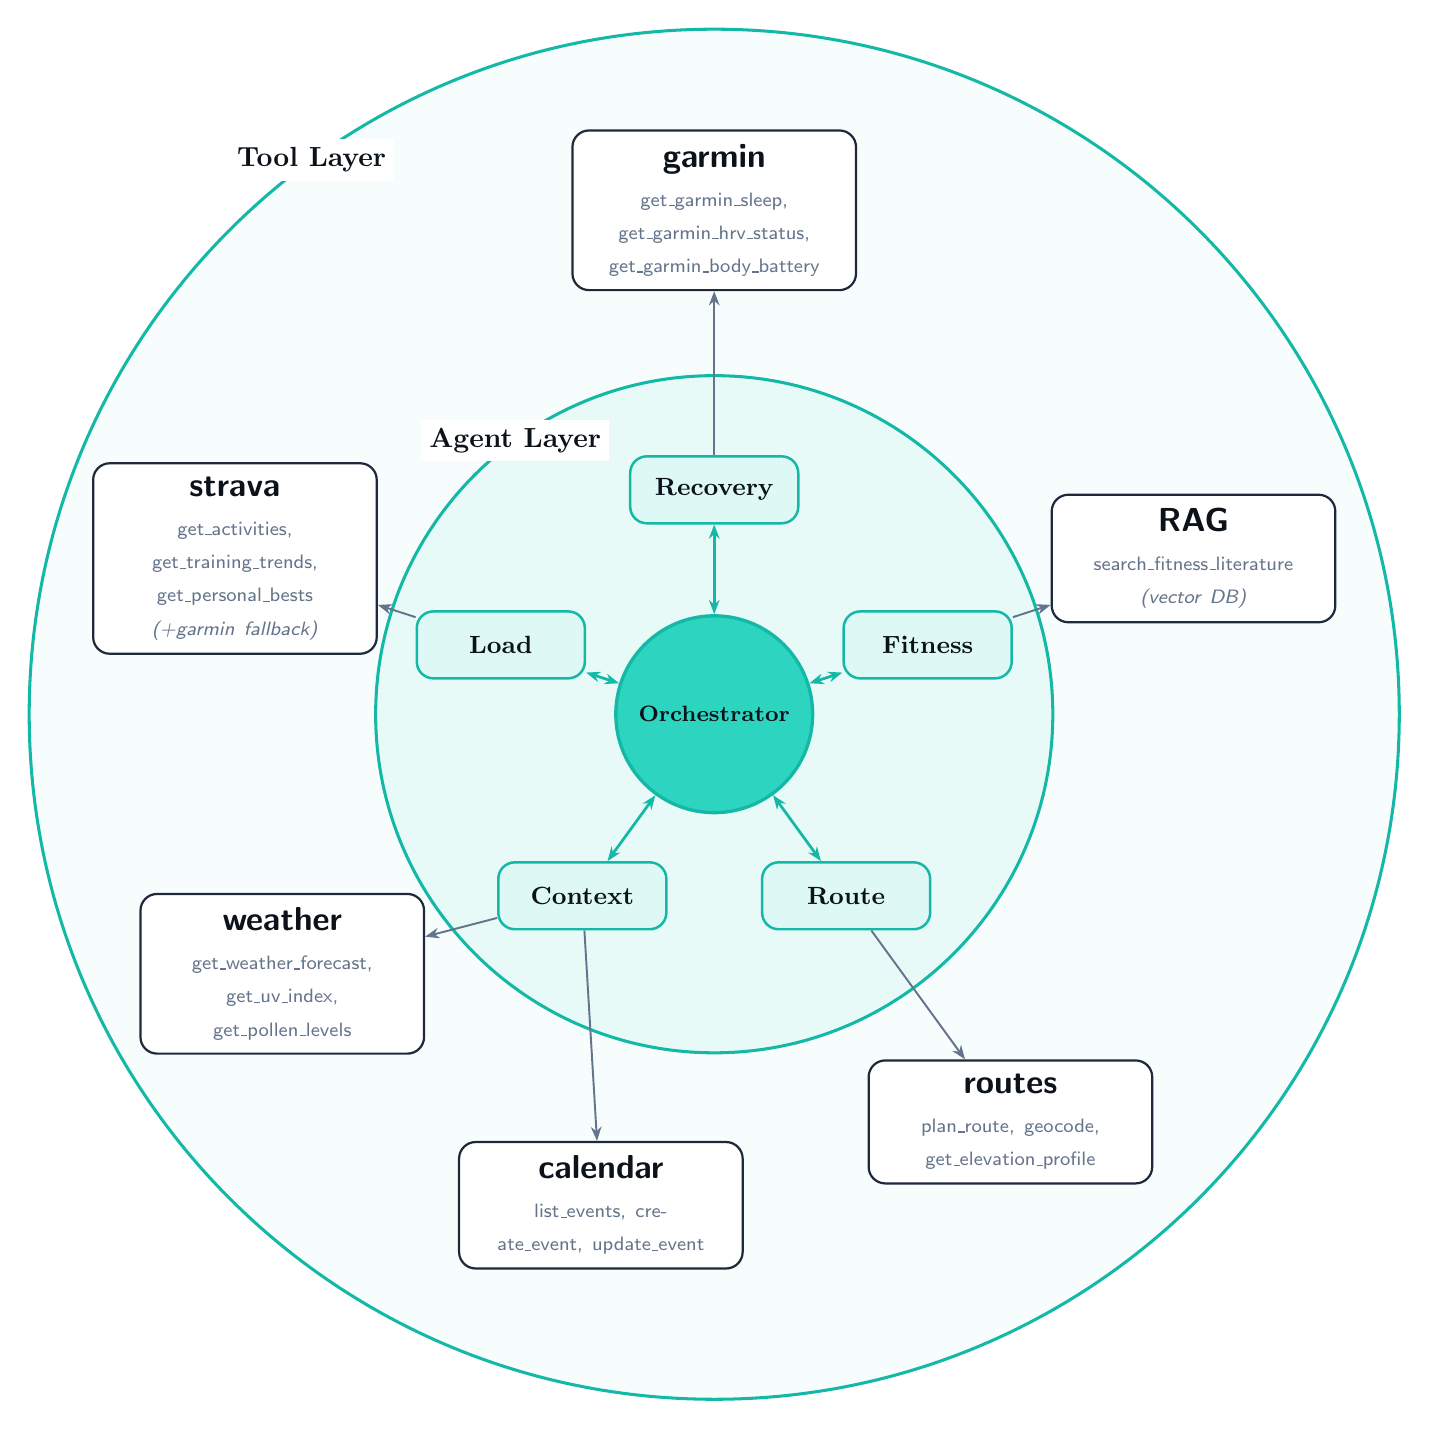
\begin{tikzpicture}[
  font=\sffamily,
  orch/.style={circle, draw=fdTealDark, line width=1.2pt, fill=fdTeal, text=fdNavy,
               font=\footnotesize\bfseries, align=center, minimum size=2.5cm},
  agent/.style={rounded corners=6pt, draw=fdTealDark, line width=0.9pt, fill=fdTeal!16,
                text=fdNavy, font=\small\bfseries, align=center, text width=1.9cm, minimum height=0.85cm},
  server/.style={rounded corners=6pt, draw=fdBorder, line width=0.8pt, fill=white, text=fdNavy,
                 align=center, text width=3.25cm, inner sep=5pt},
  ltitle/.style={font=\bfseries, text=fdNavy, fill=white, inner sep=3pt},
  a2a/.style={{Stealth[length=1.8mm]}-{Stealth[length=1.8mm]}, line width=1.0pt, draw=fdTealDark},
  uses/.style={-{Stealth[length=1.8mm]}, line width=0.7pt, draw=fdMuted},
]

% ── Centre + agents (inner ring) ─────────────────────────────────────────────
\node[orch] (orch) at (0,0) {Orchestrator};
\node[agent] (arec)  at ( 90:2.85) {Recovery};
\node[agent] (aload) at (162:2.85) {Load};
\node[agent] (actx)  at (234:2.85) {Context};
\node[agent] (arou)  at (306:2.85) {Route};
\node[agent] (afit)  at ( 18:2.85) {Fitness};

% ── MCP servers (outer ring): big name + small tool list ─────────────────────
\node[server] (sgarmin)  at ( 90:6.4) {\srv{garmin}{get\_garmin\_sleep, get\_garmin\_hrv\_status, get\_garmin\_body\_battery}};
\node[server] (sstrava)  at (162:6.4) {\srv{strava}{get\_activities, get\_training\_trends, get\_personal\_bests \textit{(+garmin fallback)}}};
\node[server] (sweather) at (211:6.4) {\srv{weather}{get\_weather\_forecast, get\_uv\_index, get\_pollen\_levels}};
\node[server] (scal)     at (257:6.4) {\srv{calendar}{list\_events, create\_event, update\_event}};
\node[server] (sroutes)  at (306:6.4) {\srv{routes}{plan\_route, geocode, get\_elevation\_profile}};
\node[server] (srag)     at ( 18:6.4) {\srv{RAG}{search\_fitness\_literature \textit{(vector DB)}}};

% ── Layer titles (on the ring outlines, in a clear gap at 126°) ──────────────
\node[ltitle] at (126:4.3) {Agent Layer};
\node[ltitle] at (126:8.7) {Tool Layer};

% ── Background: tinted disks, ring outlines, connectors ──────────────────────
\begin{scope}[on background layer]
  \fill[fdTeal!4] (0,0) circle (8.7);
  \fill[fdTeal!11] (0,0) circle (4.3);
  \draw[fdTealDark, line width=1.1pt] (0,0) circle (4.3);
  \draw[fdTealDark, line width=1.1pt] (0,0) circle (8.7);

  % Orchestrator <-> agents (A2A)
  \foreach \a in {arec,aload,actx,arou,afit}{ \draw[a2a] (orch) -- (\a); }

  % Agent -> the MCP server(s) it uses
  \draw[uses] (arec) -- (sgarmin);
  \draw[uses] (aload) -- (sstrava);
  \draw[uses] (actx) -- (sweather);
  \draw[uses] (actx) -- (scal);
  \draw[uses] (arou) -- (sroutes);
  \draw[uses] (afit) -- (srag);
\end{scope}

\end{tikzpicture}
\end{document}
